%%%%%%%%%%%%%%%%%%%%%%%%%%%%%%%%%%%%
% Slide options
%%%%%%%%%%%%%%%%%%%%%%%%%%%%%%%%%%%%

% Option 1: Slides with solutions

\documentclass[slidestop,compress,mathserif]{beamer}
\newcommand{\soln}[1]{\textit{#1}}
\newcommand{\solnGr}[1]{#1}

% Option 2: Handouts without solutions

%\documentclass[11pt,containsverbatim,handout]{beamer}
%\usepackage{pgfpages}
%\pgfpagesuselayout{4 on 1}[letterpaper,landscape,border shrink=5mm]
%\newcommand{\soln}[1]{ }
%\newcommand{\solnGr}{ }


%%%%%%%%%%%%%%%%%%%%%%%%%%%%%%%%%%%%
% Style
%%%%%%%%%%%%%%%%%%%%%%%%%%%%%%%%%%%%

\usetheme{metropolis}

%%%%%%%%%%%%%%%%
% Packages
%%%%
%%%%%% pacotes para acentos
%\usepackage[english]{babel}
%\usepackage[latin1]{inputenc}
\usepackage[utf8]{inputenc} 
\usepackage[brazil]{babel}
\usepackage[T1]{fontenc}

\usepackage{geometry}
\usepackage{graphicx}
\usepackage{amssymb}
%\usepackage{cancel}
\usepackage{epstopdf}
\usepackage{amsmath}  	% this permits text in eqnarray among other benefits
\usepackage{url}		% produces hyperlinks
\usepackage{hyperref}	% allows for color usage in tables

\usepackage{colortbl}	% allows for color usage in tables
\usepackage{multirow}	% allows for rows that span multiple rows in tables
\usepackage{color}		% this package has a variety of color options
\usepackage{pgf}
\usepackage{calc}
\usepackage{ulem}
\usepackage{multicol}
\usepackage{textcomp}
\usepackage{txfonts}
\usepackage{listings}
\usepackage{tikz}
\usepackage{array}
\usepackage{wasysym}
\usepackage{fancyvrb}
\usepackage{ragged2e} % justifica o texto
\usepackage{scalefnt} %redimensiona o tamanho da tabela comando = \scalefont{0.5}

%%%%%%%%%%%%%%%%
% Remove navigation symbols
%%%%%%%%%%%%%%%%

\setbeamertemplate{navigation symbols}{}

%%%%%%%%%%%%%%%%
% User defined colors
%%%%%%%%%%%%%%%%

\xdefinecolor{oiB}{rgb}{0.22,0.52,0.72}
\definecolor{oiG}{rgb}{.298,.447,.114}
\xdefinecolor{hlblue}{rgb}{0.051,0.65,1}
\xdefinecolor{gray}{rgb}{0.5, 0.5, 0.5}
\xdefinecolor{darkGray}{rgb}{0.3, 0.3, 0.3}
\xdefinecolor{darkerGray}{rgb}{0.2, 0.2, 0.2}
\xdefinecolor{rubineRed}{rgb}{0.89,0,0.30}
\xdefinecolor{irishGreen}{rgb}{0,0.60,0}	
\definecolor{lightGreen}{rgb}{0.387,0.581,0.148} 

%%%%%%%%%%%%%%%%
% Template colors
%%%%%%%%%%%%%%%%

%\setbeamercolor*{palette primary}{fg=white,bg= oiB!80!black!90}
%\setbeamercolor*{palette secondary}{fg=black,bg= oiB!80!black}
%\setbeamercolor*{palette tertiary}{fg=white,bg= oiB!80!black!80}
%\setbeamercolor*{palette quaternary}{fg=white,bg= oiB}
%\setbeamercolor{structure}{fg= oiB}
%\setbeamercolor{frametitle}{bg= oiB!90}
%\setbeamertemplate{blocks}[shadow=false]
%\setbeamersize{text margin left=2em,text margin right=2em}

%\setbeamercolor{code body}{bg=gray!20!white!80,fg=black}


%%%%%%%%%%%%%%%%
% Get rid of fancy enumerated list bullets
%%%%%%%%%%%%%%%%

%\setbeamertemplate{enumerate items}[default]

%%%%%%%%%%%%%%%%
% Custom commands
%%%%%%%%%%%%%%%%

% degree
\newcommand{\degree}{\ensuremath{^\circ}}

% cite
\newcommand{\ct}[1]{
\vfill
{\tiny #1}}

% Note
\newcommand{\Note}[1]{
\rule{2.5cm}{0.25pt} \\ \textit{\footnotesize{\textcolor{rubineRed}{Note:} \textcolor{darkerGray}{#1}}}}

% Remember
\newcommand{\Remember}[1]{\textit{\scriptsize{\textcolor{orange}{Remember:} #1}}}

% expected counts
\newcommand{\ex}[1]{\textit{\textcolor{blue}{#1}}}

% red
\newcommand{\red}[1]{\textit{\textcolor{rubineRed}{#1}}}

% pink
\newcommand{\pink}[1]{\textit{\textcolor{rubineRed!90!white!50}{#1}}}

% green
\newcommand{\green}[1]{\textit{\textcolor{irishGreen}{#1}}}

% orange
\newcommand{\orange}[1]{\textit{\textcolor{orange}{#1}}}

% links: webURL, webLin, appLink
\newcommand{\webURL}[1]{\urlstyle{same}{ \textit{\textcolor{darkGray}{\url{#1}}}}}
\newcommand{\webLink}[2]{\href{#1}{\textcolor{darkGray}{{#2}}}}
\newcommand{\appLink}[2]{\href{#1}{\textcolor{white}{{#2}}}}

% mail
\newcommand{\mail}[1]{\href{mailto:#1}{\textit{\textcolor{darkGray}{#1}}}}

% highlighting: hl, hlGr, mathhl
\newcommand{\hl}[1]{\textit{\textcolor{hlblue}{#1}}}
\newcommand{\hlGr}[1]{\textit{\textcolor{lightGreen}{#1}}}
\newcommand{\mathhl}[1]{\textcolor{hlblue}{\ensuremath{#1}}}

% two col: two columns
\newenvironment{twocol}[4]{
\begin{columns}[c]
\column{#1\textwidth}
#3
\column{#2\textwidth}
#4
\end{columns}
}

% slot (for probability calculations)
\newenvironment{slot}[2]{
\begin{array}{c} 
\underline{#1} \\ 
#2
\end{array}
}

% pr: left and right parentheses
\newcommand{\pr}[1]{
\left( #1 \right)
}

% solnMult: solutions for practice questions

\newcommand{\solnMult}[1]{
\item[] \vspace{-0.59cm}
\only<1>{\item #1}
\soln{\only<2->{\item \orange{#1}}}
}

% cancel
\newcommand{\cancel}[1]{%
    \tikz[baseline=(tocancel.base)]{
        \node[inner sep=0pt,outer sep=0pt] (tocancel) {#1};
        \draw[red, line width=0.5mm] (tocancel.south west) -- (tocancel.north east);
    }%
}

% removepagenumbers
\newcommand{\removepagenumbers}{% 
  \setbeamertemplate{footline}{}
}

%%%%%%%%%%%%%%%%
% Custom boxes
%%%%%%%%%%%%%%%%

% app: application exercise

\setbeamercolor{app body}{fg=oiG}

\newcommand{\app}[1]{
\begin{beamerboxesrounded}[shadow = false, lower = app body]{}
#1
\end{beamerboxesrounded}
}

% dq: discussion question

\setbeamercolor{disc ques body}{fg=oiB}

\newcommand{\dq}[1]{
\begin{beamerboxesrounded}[shadow = false, lower = disc ques body]{}
#1
\end{beamerboxesrounded}
}

% pq: practice question

\setbeamercolor{prac ques body}{fg=oiB}

\newcommand{\pq}[1]{
\begin{beamerboxesrounded}[shadow = false, lower = prac ques body]{}
#1
\end{beamerboxesrounded}
}

% formula

\setbeamercolor{formula body}{fg=oiB!55!black!95}

\newcommand{\formula}[1]{
\begin{beamerboxesrounded}[shadow = false, lower = formula body]{}
#1
\end{beamerboxesrounded}
}


%%%%%%%%%%%%%%%%
% Change margin
%%%%%%%%%%%%%%%%

\newenvironment{changemargin}[2]{%
\begin{list}{}{%
\setlength{\topsep}{0pt}%
\setlength{\leftmargin}{#1}%
\setlength{\rightmargin}{#2}%
\setlength{\listparindent}{\parindent}%
\setlength{\itemindent}{\parindent}%
\setlength{\parsep}{\parskip}%
}%
\item}{\end{list}}

%%%%%%%%%%%%%%%%
% Footnote
%%%%%%%%%%%%%%%%

\long\def\symbolfootnote[#1]#2{\begingroup%
\def\thefootnote{\fnsymbol{footnote}}\footnote[#1]{#2}\endgroup}

%%%%%%%%%%%%%%%%
% Commands from the book
%%%%%%%%%%%%%%%%

\newenvironment{data}[1]{\texttt{#1}}{}
\newenvironment{var}[1]{\texttt{#1}}{}
\newenvironment{resp}[1]{\texttt{#1}}{}

%%%%%%%%%%%%%%%%
% Graphics
%%%%%%%%%%%%%%%%

\DeclareGraphicsRule{.tif}{png}{.png}{`convert #1 `dirname #1`/`basename #1 .tif`.png}


%%%%%%%%%%%%%%%%%%%%%%%%%%%%%%%%%%%%
% Preamble
%%%%%%%%%%%%%%%%%%%%%%%%%%%%%%%%%%%%

\title[Chp 2: Probability]{Capítulo 2: Probabilidade}

\institute{$\:$ \\ {\footnotesize Slides baseados no material desenvolvido por Mine \c{C}etinkaya-Rundel of OpenIntro. 

Algumas imagens podem ser incluídas em diretrizes de uso justo (propósitos educacionais).}}
\date{}

%\author{OpenIntro Statistics, $3^0$ Edição}
%\institute{$\:$ \\ {\footnotesize Slides desenvolvidos por Mine \c{C}etinkaya-Rundel of OpenIntro. \\
%Os slides podem ser copiados, editados e / ou compartilhados via \webLink{http://creativecommons.org/licenses/by-sa/3.0/us/}{CC BY-SA license.} \\
%Algumas imagens podem ser incluídas em diretrizes de uso justo (propósitos educacionais).}}
%\date{}

%%%%%%%%%%%%%%%%%%%%%%%%%%%%%%%%%%%%
% Begin document
%%%%%%%%%%%%%%%%%%%%%%%%%%%%%%%%%%%%

\begin{document}


%%%%%%%%%%%%%%%%%%%%%%%%%%%%%%%%%%%%
% Title page
%%%%%%%%%%%%%%%%%%%%%%%%%%%%%%%%%%%%

{
\addtocounter{framenumber}{-1} 
{\removepagenumbers 
\usebackgroundtemplate{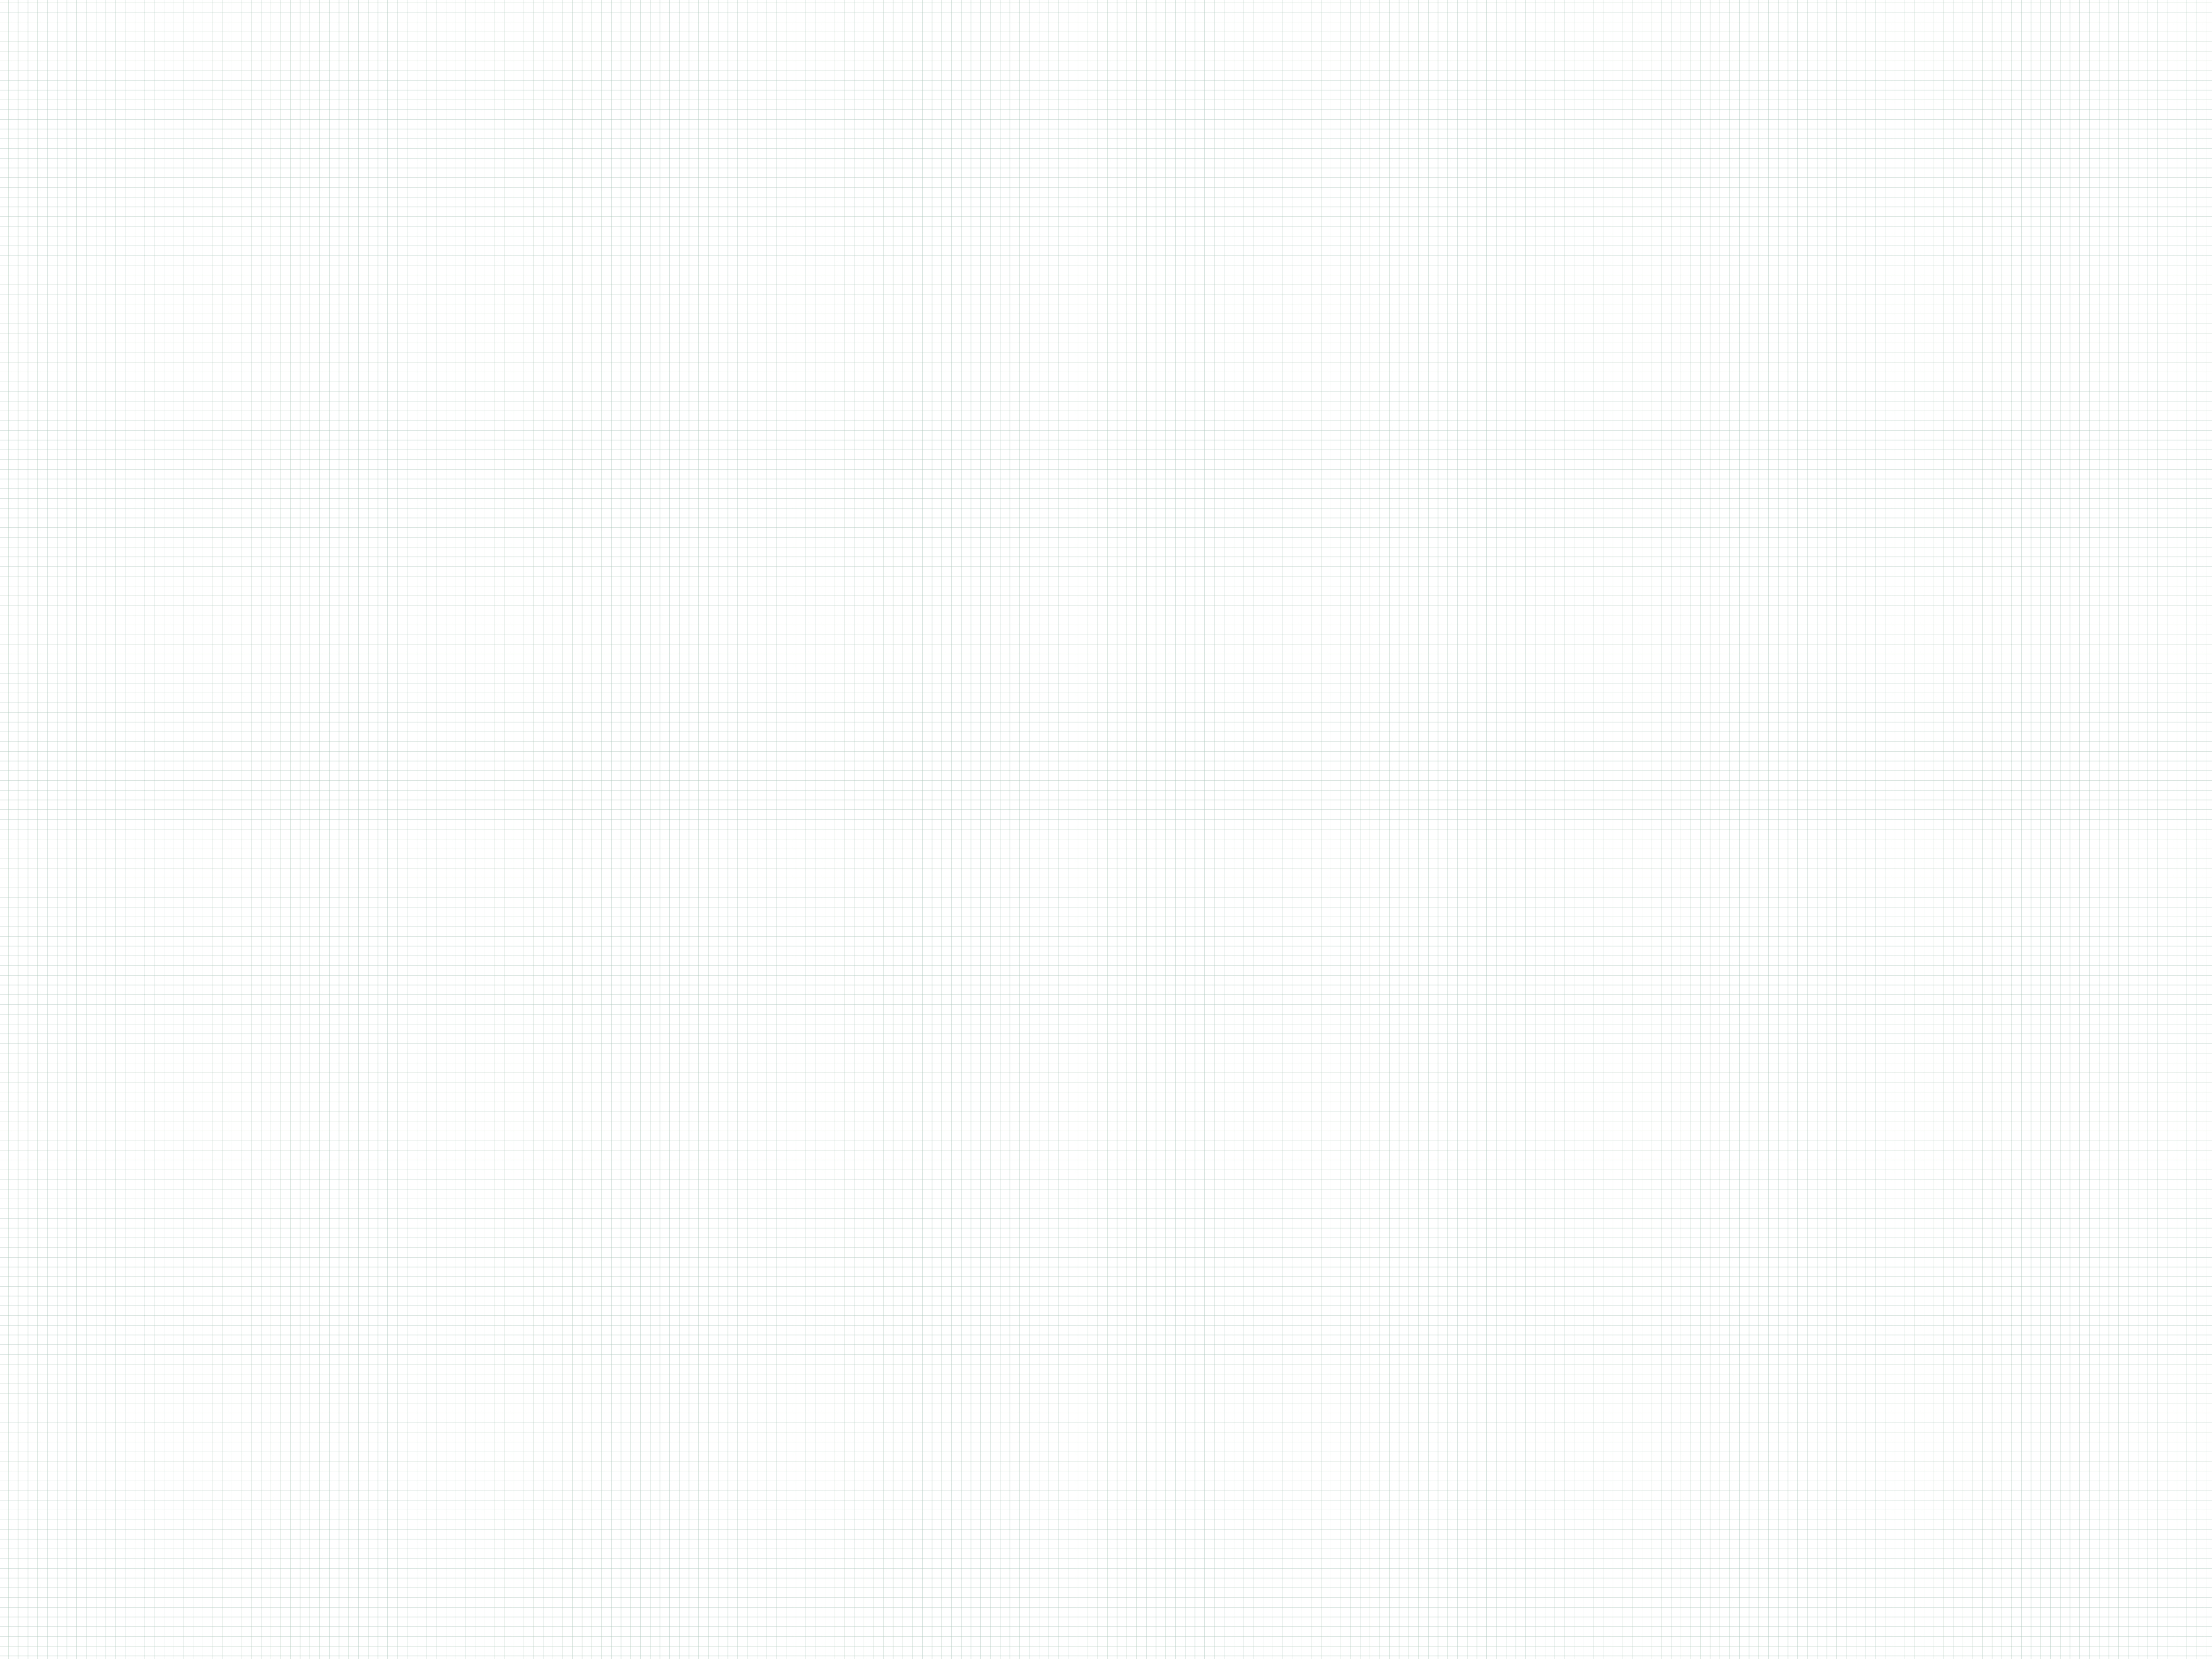
\includegraphics[width=\paperwidth]{../OpenIntro_Grid_4_3-01.jpg}}

\begin{frame}


\includegraphics[width=10cm]{../logo_ead.png}

\small	{\textit{Tradução e adaptação: }\\
Priscilla Priscilla Gnewuch e Márcia Helena Barbian}

\footnotesize{Slides baseados no material desenvolvido por Mine \c{C}etinkaya-Rundel of OpenIntro. }

\footnotesize{Tanto este material  \href{https://github.com/Probabilidade-e-Estatistica-EAD/slides_openintro}{adaptado}, quanto o \href{https://github.com/OpenIntroStat/openintro-statistics-slides}{original}, podem ser copiados, editados e/ou compartilhados. O material adaptado está licenciado sob a Licença Creative Commons Atribuição  4.0 Internacional. Para ver uma cópia desta licença, visite \href{http://creativecommons.org/licenses/by/4.0/} {http://creativecommons.org/licenses/by/4.0/}}


\hfill 
\includegraphics[width=15mm]{../ufrgs-logo}
\includegraphics[width=20mm]{../logoime}
\includegraphics[width=20mm]{../sead-logo}


\end{frame}

\begin{frame}

%\hfill 
\includegraphics[width=20mm]{../oiLogo_highres}

\titlepage

\end{frame}

}
}



%%%%%%%%%%%%%%%%%%%%%%%%%%%%%%%%%%%%
% Sections
%%%%%%%%%%%%%%%%%%%%%%%%%%%%%%%%%%%%

%%%%%%%%%%%%%%%%%%%%%%%%%%%%%%%%%%%%

\section{2.1. Definindo probabilidade}

%%%%%%%%%%%%%%%%%%%%%%%%%%%%%%%%%%%%

\subsection{Probabilidade}

%%%%%%%%%%%%%%%%%%%%%%%%%%%%%%%%%%%%

\begin{frame}
\frametitle{Processos aleatórios}

\twocol{0.5}{0.5}
{
\begin{itemize}
\justifying
\item Num \hl{processo aleatório} sabemos quais resultados \hl{podem acontecer}, mas não sabemos qual resultado específico \hl{irá acontecer}.

\end{itemize}
}{
\begin{center}
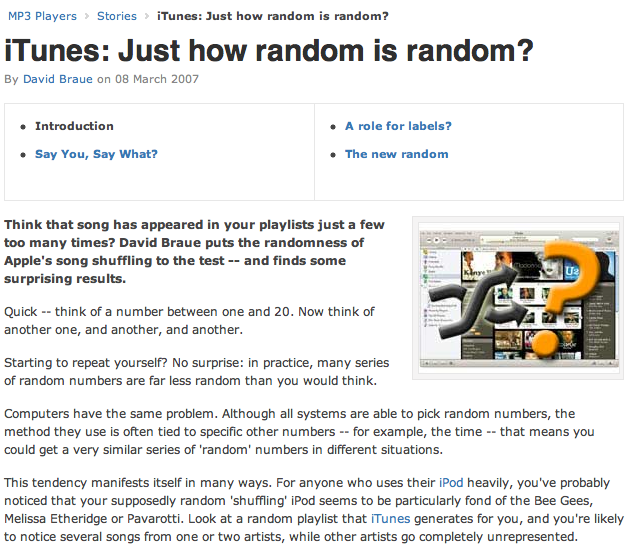
\includegraphics[width=\textwidth]{2-1_define_probability/iTunes.png}
\end{center}
\justifying
\ct{ \webURL{http://www.cnet.com.au/itunes-just-how-random-is-random-339274094.htm}}
}

\end{frame}
%%%%%%%%%%%%%%%%%%%%%%%%%%%%%%%%%%%%

\begin{frame}
\frametitle{Processos aleatórios, tradução do texto}

\justifying
\hl{iTunes: Apenas como aleatório é aleatório?}\\
\vspace{0.5cm}
\justifying
\tiny{
Acha que essa música apareceu nas suas listas de reprodução apenas algumas vezes? David Braue coloca à prova a aleatoriedade do embaralhamento de músicas da Apple - e encontra alguns resultados surpreendentes.\\
\vspace{0.1cm}
\justifying
Por David Braue 4 de agosto de 2008 20:54 AEST\\
\vspace{0.1cm}

\justifying
Rápido - pense em um número entre um e 20. Agora pense em outro, e outro, e outro.\\

\justifying
Começando a se repetir? Nenhuma surpresa: na prática, muitas séries de números aleatórios são muito menos aleatórias do que você imagina.\\
\justifying
Computadores têm o mesmo problema. Embora todos os sistemas sejam capazes de escolher números aleatórios, o método que eles usam é frequentemente vinculado a outros números específicos - por exemplo, o tempo - o que significa que você pode obter uma série muito semelhante de números "aleatórios" em diferentes situações.\\

\justifying
Essa tendência se manifesta de várias maneiras. Para qualquer um que usa streaming de música, provavelmente notou que o “aleatório”, supostamente aleatório, parece gostar particularmente dos Bee Gees, Melissa Etheridge ou Pavarotti. Olhe para uma lista de reprodução aleatória que o iTunes gera para você, e você provavelmente notará várias músicas de um ou dois artistas, enquanto outros artistas ficarão completamente sem representação.
}
\end{frame}
%%%%%%%%%%%%%%%%%%%%%%%%%%%%%%%%%%%%

\begin{frame}
\frametitle{Processos aleatórios (cont.)}

\begin{itemize}
\justifying
\item Exemplos: lançamentos de moedas, lançamentos de dados, iTunes aleatório, se o mercado de ações subir ou descer amanhã, etc.
\justifying
\item Pode ser útil modelar um processo como aleatório, mesmo que não seja verdadeiramente aleatório.

\end{itemize}
\end{frame}

%%%%%%%%%%%%%%%%%%%%%%%%%%%%%%%%%%%%

\subsection{Definindo probabilidade}

%%%%%%%%%%%%%%%%%%%%%%%%%%%%%%%%%%%%

\begin{frame}
\frametitle{Probabilidade}

\begin{itemize}
\justifying
\item Apesar de existirem diferentes interpretações possíveis de probabilidade, elas concordam  com as regras matemáticas que a probabilidade deve seguir.
\begin{itemize}
\item $P(A)$ = Probabilidade do evento A
\item $0 \le P(A) \le 1$
\end{itemize}

\pause
\justifying
\item \hl{Interpretação Frequentista:} 
\begin{itemize}
\justifying
\item A probabilidade de um resultado é a proporção de vezes que o resultado ocorreria se observássemos o processo aleatório um número infinito de vezes.
\end{itemize}
\end{itemize}

\pause
\end{frame}
%%%%%%%%%%%%%%%%%%%%%%%%%%%%%%%%%%%%

\begin{frame}
\frametitle{Probabilidade}

\begin{itemize}
\justifying
\item \hl{Interpretação Bayesiana:} 
\begin{itemize}
\justifying
\item  Um bayesiano interpreta probabilidade como um grau subjetivo de crença: para o mesmo evento, duas pessoas separadas poderiam ter pontos de vista diferentes e, assim, atribuir probabilidades diferentes.
\justifying
\item Amplamente popularizado pelo avanço revolucionário em métodos computacionais e tecnologia.
\end{itemize}

\end{itemize}

\end{frame}

%%%%%%%%%%%%%%%%%%%%%%%%%%%%%%%%%%%%

\begin{frame}
\frametitle{Prática}
\frametitle{Prática}
\justifying
\pq{Você se surpreenderia mais com qual dos seguintes eventos?}

\begin{enumerate}[(a)]
\justifying
\item exatamente 3 coroas em 10 lançamentos de uma moeda.
\justifying
\item exatamente 3 coroas em 100 lançamentos consecutivos de uma moeda.
\justifying
\solnMult{exatamente 3 coroas em 1000 lançamentos consecutivos de uma moeda.}
\end{enumerate}

\end{frame}

%%%%%%%%%%%%%%%%%%%%%%%%%%%%%%%%%%%%

\begin{frame}
\frametitle{Lei dos grandes números}
\justifying
\hl{Lei de grandes números} afirma que à medida que mais observações são coletadas, a proporção de ocorrências de um determinado resultado, \mathhl {\hat {p} _n}, converge para a probabilidade desse resultado, \mathhl {p}.

\end{frame}

%%%%%%%%%%%%%%%%%%%%%%%%%%%%%%%%%%%%

\begin{frame}
\frametitle{Lei dos grandes números (cont.)}
\justifying
\dq{Imagine que em lançamentos consecutivos de uma uma moeda \textit{não viciada}, apareçam cara nos 10 primeiros arremessos. Você apostaria que a chance de aparecer cara no próximo lance é? 0,5, menor que 0,5 ou maior que 0,5?}
\[ \underline{H} \hspace{1mm} \underline{H} \hspace{1mm} \underline{H} \hspace{1mm} \underline{H} \hspace{1mm} \underline{H} \hspace{1mm} \underline{H} \hspace{1mm} \underline{H} \hspace{1mm} \underline{H} \hspace{1mm} \underline{H} \hspace{1mm} \underline{H} \hspace{1mm} \underline{?} \]
\small{
\begin{itemize}
\justifying
\item<2-> A probabilidade ainda é de 0,5, ou seja, ainda há 50\% de chance de que outra cara apareça no próximo lançamento.
\[ P(H \text{ em 11}^{0} \text{ sorteio}) = P(T \text{ em 11}^{0} \text{ sorteio}) = 0.5 \]
\end{itemize}
}
\end{frame}
%%%%%%%%%%%%%%%%%%%%%%%%%%%%%%%%%%%%

\begin{frame}
\frametitle{Lei de grandes números (cont.)}
\justifying

\begin{itemize}
\item  A moeda não  "lembra" o que aconteceu, ela não é influenciada pela quantidade de caras observadas.
\justifying
\item Uma interpretação equivocada da Lei dos Grandes Números é que processos aleatórios devem compensar o que aconteceu no passado; isso não é verdade, essa idéia incorreta é conhecida como \hl{falácia do jogador}.
\end{itemize}

\end{frame}

%%%%%%%%%%%%%%%%%%%%%%%%%%%%%%%%%%%%

\subsection{Mutuamente exclusivos}

%%%%%%%%%%%%%%%%%%%%%%%%%%%%%%%%%%%%

\begin{frame}
\frametitle{Eventos disjuntos}
\justifying
\hl{Eventos disjuntos:} Não podem acontecer ao mesmo tempo.
\begin{itemize}
\justifying
\item O resultado de um único lançamento da moeda não pode ser uma cara e uma coroa ao mesmo tempo.
\justifying
\item Um aluno não pode reprovar e ser aprovado em uma disciplina.
\justifying
\item Uma única carta tirada de um baralho não pode ser um ás e uma dama.
\justifying
\item O resultado de um exame não pode ser positivo \hl{e} negativo.
\justifying
\item A cor de um carro, pode apresentar vários resultados, todos disjuntos.
\end{itemize}

\pause
\justifying
\hl{Eventos não disjuntos:} Podem acontecer ao mesmo tempo.
\begin{itemize}
\justifying
\item Um estudante pode obter um conceito A em Estatística e A em Física no mesmo semestre.
\end{itemize}

\end{frame}

%%%%%%%%%%%%%%%%%%%%%%%%%%%%%%%%%%%%

\begin{frame}
\frametitle{União de eventos}
\justifying
\dq{Qual é a probabilidade de tirar um valete ou uma carta vermelha de um baralho completo bem embaralhado?}

\begin{figure}
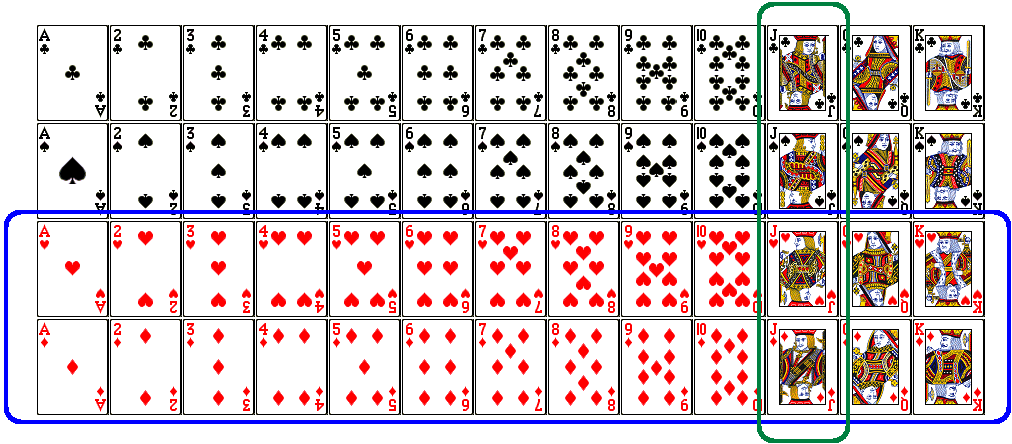
\includegraphics[width=0.7\textwidth]{2-1_define_probability/cards.png}
\end{figure}

\vspace{-0.75cm}

\soln{\onslide<2->{
\begin{align*}
P(valete~ou~vermelho) &= P(valete) + P(vermelho) - \orange{$P(valete~e~vermelho)$} \\
&= \frac{4}{52} + \frac{26}{52} - \frac{2}{52} = \frac{28}{52}
\end{align*}
}}

\vfill

\ct{Figure from \webURL{http://www.milefoot.com/math/discrete/counting/cardfreq.htm}.}

\end{frame}

%%%%%%%%%%%%%%%%%%%%%%%%%%%%%%%%%%%%

\subsection{Probabilidade}

%%%%%%%%%%%%%%%%%%%%%%%%%%%%%%%%%%%%

\begin{frame}
\frametitle{Prática}
\justifying
\pq{Qual a probabilidade de um estudante selecionado aleatoriamente ter a opinião de que a maconha deve ser legalizada \underline{ou} concordar com as opiniões políticas de seus pais?}

{\small
\begin{center}
\begin{tabular}{l  cc c}
            & \multicolumn{2}{c}{\textit{Compartilha a opinião política dos pais}} & \\
\cline{2-3}
\textit{A favor da Legalização} & Não & Sim & Total \\
\hline
Não          & 11 & 40 & 51 \\
Sim         & 36 & 78 & 114 \\
\hline
Total       & 47 & 118 & 165
\end{tabular}
\end{center}
}

\begin{enumerate}[(a)]
\item $\frac{40 + 36 - 78}{165}$
\solnMult{$\frac{114 + 118 - 78}{165}$}
\item $\frac{78}{165}$
\item $\frac{78}{188}$
\item $\frac{11}{47}$
\end{enumerate}

\end{frame}

%%%%%%%%%%%%%%%%%%%%%%%%%%%%%%%%%%%%

\begin{frame}
\frametitle{União de eventos}
\justifying
\formula{Regra da adição}{\[ P(A~ou~B) = P(A) + P(B) - P(A~e~B) \]}
\[ P(A\cup B) = P(A) + P(B) - P(A\cap B) \]
\justifying
\Note{Para eventos disjuntos $P(A~e~B) = 0$, então a fórmula acima será simplificada para $P(A~ou~B) = P(A) + P(B)$.}

\end{frame}

%%%%%%%%%%%%%%%%%%%%%%%%%%%%%%%%%%%%

\subsection{Distribuições de probabilidade}

%%%%%%%%%%%%%%%%%%%%%%%%%%%%%%%%%%%%

\begin{frame}
\frametitle{Distribuição de probabilidade}
\justifying
Uma \hl{distribuição de probabilidade} lista todos os eventos possíveis e as probabilidades com as quais eles ocorrem.

\begin{itemize}
\justifying
\item A distribuição de probabilidade para o resultado do arremesso de uma moeda não viciada:
{\footnotesize 
\begin{center}
\begin{tabular}{r | c | c}
Evento    & Cara (C)		& Coroa (K) \\
\hline
Probabilidade	& 0.5		& 0.5 \\
\end{tabular}
\end{center}
}
\vspace{0.1cm}
\pause
\justifying
\item Regras de uma distribuição de probabilidade:
\begin{enumerate}
\justifying
\item Os eventos listados não podem ocorrer ao mesmo tempo.
\justifying
\item Cada probabilidade deve estar entre 0 e 1.
\justifying
\item As probabilidades somadas devem totalizar 1.
\end{enumerate}

\pause
\justifying
\item A distribuição de probabilidade para o resultado do arremesso de duas moedas:
\soln{
\only<2->{
{\footnotesize
\begin{center}
\begin{tabular}{r | c | c | c | c}
Evento		& CC	& KK		& CK		& KC \\
\hline
Probabilidade	& 0.25	& 0.25	& 0.25	& 0.25 \\
\end{tabular}
\end{center}
}}}

\end{itemize}

\end{frame}

%%%%%%%%%%%%%%%%%%%%%%%%%%%%%%%%%%%%

\begin{frame}
\frametitle{Prática}
\justifying
\pq{Em uma pesquisa, 52\% dos entrevistados disseram que são gremistas. Qual é a probabilidade de que um respondente selecionado aleatoriamente desta amostra seja colorado?}

\begin{enumerate}[(a)]
\justifying
\item 0.48
\justifying
\item mais de 0.48
\justifying
\item menos de 0.48
\justifying
\solnMult{Não pode ser calculada usando apenas a informação dada}\\
\end{enumerate}
\justifying
\soln{\only<2>{\orange{Se há somente dois times, o Grêmio e o Inter, então (a) é possível. No entanto, pode ser que algumas pessoas não torçam pra nenhum time ou que sejam torcedores de outro clube. Então (c) também é possível. A letra (b) não pode ser a resposta, uma vez que a probabilidade seria superior a 1.}}}

\end{frame}

%%%%%%%%%%%%%%%%%%%%%%%%%%%%%%%%%%%%

%%%%%%%%%%%%%%%%%%%%%%%%%%%%%%%%%%%%

\subsection{Complemento de um evento}

%%%%%%%%%%%%%%%%%%%%%%%%%%%%%%%%%%%%

\begin{frame}
\frametitle{Espaço amostral}
\justifying
\hl{Espaço amostral} é a coleção de todos os resultados possíveis de um estudo.

\begin{itemize}
\justifying
\item Um casal tem um filho, qual é o espaço amostral para o sexo da criança? $S = \{ M, F \}$.
\justifying
\item Um casal tem dois filhos, qual é o espaço amostral para o sexo dessas crianças? \soln{\pause{$S = \{ MM, FF, FM, MF \}$}}
\end{itemize}

\pause

\end{frame}
%%%%%%%%%%%%%%%%%%%%%%%%%%%%%%%%%%%%

\begin{frame}
\frametitle{Evento complementar}

\justifying
\hl{Eventos complementares} são dois eventos mutuamente exclusivos cujas probabilidades somam 1.

\begin{itemize}
\justifying
\item Um casal tem um filho. Se sabemos que a criança não é um menino, qual é o sexo dessa criança?
\justifying
\{ \sout{\textcolor{gray}{M}}, \orange{F} \} $\rightarrow$ menino e menina são resultados \hl{complementares}.
\justifying
\item Um casal tem dois filhos, se sabemos que eles não são meninas, quais são as possíveis combinações de gênero para essas crianças?
\soln{\pause{\{ \orange{MM}, \sout{\textcolor{gray}{FF}}, \orange{FM}, \orange{MF} \} }}
\end{itemize}

\end{frame}

%%%%%%%%%%%%%%%%%%%%%%%%%%%%%%%%%%%%

\subsection{Independência}

%%%%%%%%%%%%%%%%%%%%%%%%%%%%%%%%%%%%

\begin{frame}
\frametitle{Independência}
\justifying
Dois processos são \hl{independentes} se o resultado de um não fornecer informações úteis sobre o resultado do outro.

\pause

\begin{itemize}
\justifying
\justifying
\item Sabendo que o resultado do primeiro lançamento da moeda foi cara, \underline{isso não é} uma informação útil para determinar em que lado a moeda cairá no segundo lançamento. $\rightarrow$ Os resultados de dois lançamentos de uma moeda são independentes.

\pause
\justifying
\item Sabendo que a primeira carta tirada de um baralho é um ás, \underline{é fornecida uma informação útil} para determinar a probabilidade da segunda carta ser um ás. $\rightarrow$ Os resultados da seleção (sem reposição) de duas cartas de um baralho são dependentes.

\end{itemize}

\end{frame}

%%%%%%%%%%%%%%%%%%%%%%%%%%%%%%%%%%%%

\begin{frame}
\frametitle{Prática}
\justifying
\pq{\small{Entre os dias 9 e 12 de janeiro de 2013, a SurveyUSA entrevistou uma amostra aleatória de 500 moradores de NC, a pergunta era: permitir a posse de armas protege os cidadãos que respeitam a lei, ou torna a sociedade mais perigosa. 58\% de todos os entrevistados disseram que protege os cidadãos. 67\% dos entrevistados brancos, 28\% dos entrevistados negros e 64\% dos entrevistados hispânicos compartilharam essa visão. Qual das alternativas abaixo é verdadeira?}}
\justifying
A opinião sobre posse de armas e raça/etnia são
\begin{enumerate}[(a)]
\item complementares
\item Mutualmente exclusivas
\item independentes
\solnMult{dependentes}
\item disjuntas
\end{enumerate}
\justifying
\ct{\webURL{http://www.surveyusa.com/client/PollReport.aspx?g=a5f460ef-bba9-484b-8579-1101ea26421b}}

\end{frame}

%%%%%%%%%%%%%%%%%%%%%%%%%%%%%%%%%%%%

\begin{frame}
\frametitle{Prática}
\justifying
\formula{Verificando a independência}{Se P(A ocorre, dado que B é verdade) = $P(A~|~B) = P(A)$, então A e B são independentes.}

$\:$ \\

\soln{\pause{P(protege os cidadãos) = 0.58 \\
\pause
$\:$ \\
\justifying
P(opinião de que posse de armas protege os cidadãos, dado que o residente é branco) = \\ P(protege os cidadãos $|$ branco) = 0.67 \\
$\:$ \\
P(protege os cidadãos $|$ negro) = 0.28 \\
$\:$ \\
P(protege os cidadãos $|$ hispânico) = 0.64 \\
$\:$ \\
\pause
\justifying
P(protege os cidadãos) varia de acordo com a raça/etnia, portanto, a opinião sobre a posse de armas e raça/etnia devem ser dependentes.
}}

\end{frame}

%%%%%%%%%%%%%%%%%%%%%%%%%%%%%%%%%%%%

\begin{frame}
\frametitle{Determinando a dependência com base em dados amostrais}

\begin{itemize}
\justifying
\item Se as probabilidades condicionais calculadas com base nos dados da amostra sugerem dependência entre duas variáveis, o próximo passo é conduzir um teste de hipóteses para determinar se a diferença observada entre as probabilidades é provável ou improvável de ter ocorrido.
\justifying
\item Se a diferença observada entre as probabilidades condicionais for grande, então há evidências mais fortes de que a diferença é real.
\end{itemize}
\end{frame}

%%%%%%%%%%%%%%%%%%%%%%%%%%%%%%%%%%%%

\begin{frame}
\frametitle{Determinando a dependência com base em dados amostrais}

\begin{itemize}
\justifying
\item Se uma amostra é grande, então até mesmo uma pequena diferença pode fornecer forte evidência de uma diferença real.

\end{itemize}

\pause
\justifying
\dq{{\small Vimos que P(protege os cidadãos $|$ branco) = 0.67 e P(protege os cidadãos $|$ hispânico) = 0.64. Sob qual condição você estaria mais convencido de uma diferença real entre as proporções de brancos e hispânicos que acham que a posse de armas protege os cidadãos? $n = 500$ ou $n = 50,000$}} \pause \soln{$n = 50,000$}

\end{frame}

%%%%%%%%%%%%%%%%%%%%%%%%%%%%%%%%%%%%

\begin{frame}
\frametitle{Regra do produto para eventos independentes}
\justifying
\formula{Regra do produto para eventos independentes}{\[P(A~e~B) = P(A) \times P(B) \]
\small{Ou mais geralmente, $P(A_1~e~\cdots~e~A_k) = P(A_1) \times \cdots \times P(A_k)$}}

\pause
\justifying
\dq{Você joga uma moeda duas vezes, qual é a probabilidade de observar duas coroas seguidas?}

\pause
\justifying
\[ P(\text{Coroa no primeiro lance}) \times  P(\text{Coroa no segundo lance}) = \frac{1}{2} \times \frac{1}{2} = \frac{1}{4} \]

\end{frame}

%%%%%%%%%%%%%%%%%%%%%%%%%%%%%%%%%%%%

\begin{frame}
\frametitle{Prática}
\justifying
\pq{Uma pesquisa recente da Gallup sugere que 25,5\% dos texanos não têm plano de saúde, a pesquisa foi realizada em junho de 2012. Supondo que a proporção de pessoas sem seguro permaneça constante, qual é a probabilidade de que dois texanos selecionados aleatoriamente não tenham seguro?}

\twocol{0.4}{0.6}
{
\begin{enumerate}[(a)]
\item $25.5^2$
\solnMult{ $0.255^2$ }
\item $0.255 \times 2$
\item $(1 - 0.255)^2$
\end{enumerate}
}
{
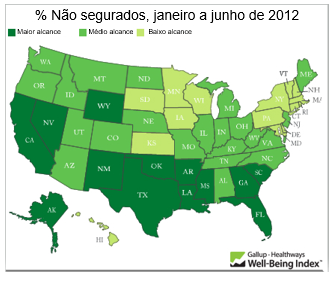
\includegraphics[width=0.9\textwidth]{2-1_define_probability/uninsured.png}
}
\justifying
\ct{ \webURL{http://www.gallup.com/poll/156851/uninsured-rate-stable-across-states-far-2012.aspx}}

\end{frame}

%%%%%%%%%%%%%%%%%%%%%%%%%%%%%%%%%%%%

\subsection{Recapitulando}

%%%%%%%%%%%%%%%%%%%%%%%%%%%%%%%%%%%%

\begin{frame}
\frametitle{Disjuntos vs. complementares}
\justifying
\dq{A soma das probabilidades de dois eventos disjuntos sempre somam 1?}

\pause
\justifying
\soln{Não necessariamente, pode haver mais de dois eventos no espaço amostral, por exemplo, times de futebol.}

\pause
$\:$ \\
\justifying
\dq{A soma das probabilidades de dois eventos complementares sempre somam 1?}

\pause
\justifying
\soln{Sim, essa é a definição de complementar, por exemplo, cara e coroa. }

\end{frame}

%%%%%%%%%%%%%%%%%%%%%%%%%%%%%%%%%%%%

\begin{frame}
\frametitle{Voltando ao exemplo do plano de saúde}
\justifying
\dq{Se fôssemos selecionar aleatoriamente 5 texanos, qual é a probabilidade de que pelo menos um não tenha plano de saúde?}

\begin{itemize}
\justifying
\item Se fôssemos selecionar aleatoriamente 5 texanos, o espaço amostral do número de texanos que não têm seguro seria:
\[ S = \{0, 1, 2, 3, 4, 5\} \]
\justifying
\item Estamos interessados em casos em que pelo menos uma pessoa não tem seguro:
\[ S = \{0, \orange{$1, 2, 3, 4, 5$} \} \]
\justifying
\item Então, podemos dividir o espaço amostral em duas categorias:
\[ S = \{0, \orange{pelo~menos~um} \} \]

\end{itemize}

\end{frame}

%%%%%%%%%%%%%%%%%%%%%%%%%%%%%%%%%%%%

\begin{frame}
\frametitle{Voltando ao exemplo do plano de saúde}
\justifying
A probabilidade do espaço amostral deve totalizar 1:
\begin{eqnarray*}
Prob (pelo~ menos ~ 1 ~ sem ~seguro) &=& 1 - Prob (nenhum ~ sem ~seguro) \\
\pause
&=& 1 - [(1-0.255)^5] \\
\pause
&=& 1- 0.745^5 \\
\pause
&=& 1 - 0.23 \\
\pause
&=& 0.77
\end{eqnarray*}

$\:$ \\
$\:$ \\
\justifying
\formula{Pelo menos 1}{\[P(pelo~ menos ~ um) = 1 - P(Nenhum)\]}

\end{frame}

%%%%%%%%%%%%%%%%%%%%%%%%%%%%%%%%%%%%

\begin{frame}
\frametitle{Prática}
\justifying
\pq{Aproximadamente 20\% dos alunos de graduação são vegetarianos ou veganos. Qual é a probabilidade de que, numa amostra aleatória de 3 universitários, pelo menos um seja vegetariano ou vegano?}

\twocol{0.3}{0.6}{
\begin{enumerate}[(a)]
\item $1 - 0.2 \times 3$
\item $1 - 0.2^3$
\item $0.8^3$
\item $1 - 0.8 \times 3$
\solnMult{$1 - 0.8^3$}
\end{enumerate}
}
{
\soln{ \only<2>{
$P(pelo~menos~1~ser~veg) = 1- P(\textit{não}~veg)$ \\
$= 1 - (1 - 0.2)^3$ \\
$= 1 - 0.8^3$ \\
$= 1 - 0.512 = 0.488$ }}
}

\end{frame}

%%%%%%%%%%%%%%%%%%%%%%%%%%%%%%%%%%%%



%%%%%%%%%%%%%%%%%%%%%%%%%%%%%%%%%%%%

\section{2.2. Probabilidade Condicional}

%%%%%%%%%%%%%%%%%%%%%%%%%%%%%%%%%%%%

\subsection{Probabilidades marginais e conjuntas}

%%%%%%%%%%%%%%%%%%%%%%%%%%%%%%%%%%%%

\begin{frame}
\frametitle{Tipos de tratamento para vício em cocaína}
\justifying
Pesquisadores distribuíram aleatoriamente 72 usuários de cocaína em três grupos de tratamento contra o vício: um grupo recebe o medicamento desipramina (antidepressivo), outro o lítio (tratamento padrão para cocaína) e o último grupo recebe um placebo. Os resultados do estudo estão resumidos abaixo.

{\small
\begin{center}
\begin{tabular}{l | c c | c}
			& 		& Não 		&  \\
			& Recaída	& Recaída	& total \\
\hline
desipramina	& 10		& 14		& 24 \\
lítio		& 18		& 6		& 24 \\
placebo		& 20		& 4		& 24 \\
\hline
total			& 48		& 24		& 72
\end{tabular}
\end{center}
}
\justifying
\ct{\webURL{http://www.oswego.edu/~srp/stats/2_way_tbl_1.htm}}

\end{frame}

%%%%%%%%%%%%%%%%%%%%%%%%%%%%%%%%%%%%

\begin{frame}
\frametitle{Probabilidade Marginal}
\justifying
\dq{Qual é a probabilidade de um paciente ter uma recaída?}

{\small
\begin{center}
\begin{tabular}{l | c c | c}
			& Ter		& Não ter 		&  \\
			& recaída	& recaída	& total \\
\hline
desipramina	& 10		& 14		& 24 \\
lítio		& 18		& 6		& 24 \\
placebo		& 20		& 4		& 24 \\
\hline
total			& \only<1>{48}\only<2->{\red{48}}		& 24		&  \only<1>{72}\only<2->{\red{72}}
\end{tabular}
\end{center}
}
\justifying
\onslide<2->{P(Ter uma recaída) = $\frac{48}{72} \approx 0.67$} \\

\end{frame}

%%%%%%%%%%%%%%%%%%%%%%%%%%%%%%%%%%%%

\begin{frame}
\frametitle{Probabilidade conjunta}
\justifying
\dq{Qual é a probabilidade de um paciente receber o antidepressivo (desipramina)? \underline{e} ter uma recaída?}

{\small
\begin{center}
\begin{tabular}{l | c c | c}
			& 		& não 		&  \\
			& recaída	& recaída	& total \\
\hline
desipramina	& \only<1>{10} \only<2->{\red{10}}		& 14		& 24 \\
lítio		& 18		& 6		& 24 \\
placebo		& 20		& 4		& 24 \\
\hline
total			& 48	& 24		&  \only<1>{72} \only<2->{\red{72}}
\end{tabular}
\end{center}
}
\justifying
\onslide<2->{P(recaída e desipramina) = $\frac{10}{72} \approx 0.14$} \\

\end{frame}

%%%%%%%%%%%%%%%%%%%%%%%%%%%%%%%%%%%%

\subsection{Definindo probabilidade condicional}

%%%%%%%%%%%%%%%%%%%%%%%%%%%%%%%%%%%%

\begin{frame}
\frametitle{Probabilidade Condicional}
\justifying
\formula{Probabilidade Condicional}{
A probabilidade do evento $A$ dado que o evento $B$ ocorreu é calculada como
\[ P(A|B) = \frac{P(A~e~B)}{P(B)} = \frac{P(A~\cap~B)}{P(B)} \]
}

\pause

\twocol{0.5}{0.5}
{
{\small
\begin{center}
\begin{tabular}{l | c c | c}
			& 		& não 		&  \\
			& recaída	& recaída	& total \\
\hline
desipramina	& 10		& 14		& 24 \\
lítio		& 18		& 6		& 24 \\
placebo		& 20		& 4		& 24  \\
\hline
total			& 48		& 24		&  72
\end{tabular}
\end{center}
}
}
{
\begin{eqnarray*}
&&P(\mbox{recaída} |  \mbox{desipramina}) \\
&&= \frac{P(\mbox{recaida} ~e ~\mbox{desipramina})}{P(\mbox{desipramina})} \\
\pause
&&= \frac{10 / 72}{24 / 72} \\
\pause
&&= \frac{10}{24} \\
\pause
&&= 0.42
\end{eqnarray*}
}

\end{frame}

%%%%%%%%%%%%%%%%%%%%%%%%%%%%%%%%%%%%

\begin{frame}
\frametitle{Probabilidade Condicional (cont.)}
\justifying
\dq{Se sabemos que um paciente recebeu o antidepressivo (desipramina), qual é a probabilidade de que ele tenha uma recaída e volte a usar a droga?}

{\small
\begin{center}
\begin{tabular}{l | c c | c}
			& 		& não 		&  \\
			& recaída	& recaída	& total \\
\hline
\rowcolor[gray]{.7}
desipramina	& \only<1>{10} \only<2->{\red{10}}			& 14		& \only<1>{24} \only<2->{\red{24}} \\
lítio		& 18		& 6		& 24 \\
placebo		& 20 		& 4		& 24  \\
\hline
total			& 48	& 24		&  72
\end{tabular}
\end{center}
}
\justifying
\onslide<2->{P(recaída $|$  desipramina) = $\frac{10}{24} \approx 0.42$} \\

\onslide<3->{
$\:$ \\
P(recaída $|$  lítio) = $\frac{18}{24} \approx 0.75$ \\
P(recaída $|$  placebo) = $\frac{20}{24} \approx 0.83$ \\
}

\end{frame}

%%%%%%%%%%%%%%%%%%%%%%%%%%%%%%%%%%%%

\begin{frame}
\frametitle{Probabilidade Condicional (cont.)}
\justifying
\dq{Se sabemos que um paciente teve uma recaída, qual é a probabilidade de terem recebido o tratamento com o antidepressivo (desipramina)?}

{\small
\begin{center}
\begin{tabular}{l | >{\columncolor[gray]{0.7}[0pt]}c c | c}
			& 		& não 		&  \\
			& recaída	& recaída	& total \\
\hline
desipramina	& \only<1>{10} \only<2->{\red{10}}			& 14		& 24 \\
lítio		& 18		& 6		& 24 \\
placebo		& 20		& 4		& 24  \\
\hline
total			& \only<1>{48} \only<2->{\red{48}}	& 24		&  72
\end{tabular}
\end{center}
}
\justifying
\onslide<2->{P(desipramina $|$  recaída) = $\frac{10}{48} \approx 0.21$} \\

\onslide<3->{
$\:$ \\
P(lítio $|$  recaída) = $\frac{18}{48} \approx 0.375$ \\
P(placebo $|$  recaída) = $\frac{20}{48} \approx 0.42$ \\
}

\end{frame}

%%%%%%%%%%%%%%%%%%%%%%%%%%%%%%%%%%%%

\subsection{Regra geral de multiplicação}

%%%%%%%%%%%%%%%%%%%%%%%%%%%%%%%%%%%%

\begin{frame}
\frametitle{Regra geral da multiplicação}

\begin{itemize}
\justifying
\item Anteriormente, vimos que, se dois eventos são independentes, a probabilidade conjunta (eles ocorrerem simultaneamente) é simplesmente o produto de suas probabilidades. Se os eventos não forem considerados independentes, a probabilidade conjunta é calculada de forma ligeiramente diferente.

\pause
\justifying
\item Se $A$ e $B$ representam dois eventos quaisquer, então
\formula{\[ P(A~e~B) = P(A|B) \times P(B) \]}
\formula{\[ P(A\cap B) = P(A|B) \times P(B) \]}

\justifying
Note que a equação acima é simplesmente a fórmula da probabilidade condicional, rearranjada.
\pause
\justifying
\item É útil pensar em $A$ como resultado e o evento $B$ como condição.

\end{itemize}

\end{frame}

%%%%%%%%%%%%%%%%%%%%%%%%%%%%%%%%%%%%

\subsection{Independência e probabilidade condicional}

%%%%%%%%%%%%%%%%%%%%%%%%%%%%%%%%%%%%

\begin{frame}
\frametitle{Probabilidade condicional}
\justifying
Considere a seguinte distribuição (hipotética) de número de alunos aprovados e reprovados nos cursos de estatística e física:

{\small
\begin{center}
\begin{tabular}{l | c c | c}

			& Estatística	& Física	& total \\
\hline
Aprovado		& 30		& 20		& 50 \\
reprovado			& 30		& 20		& 50 \\
\hline
total			& 60		& 40		& 100
\end{tabular}
\end{center}
}

\pause

\begin{itemize}
\justifying
\item A probabilidade de que um estudante selecionado aleatoriamente seja do curso da estatística é \pause $\frac{60}{100} = 0.6$. 
\end{itemize}
\end{frame}
%%%%%%%%%%%%%%%%%%%%%%%%%%%%%%%%%%%%

\begin{frame}
\frametitle{Probabilidades de eventos independentes e probabilidade condicional}
\pause
\justifying
\begin{itemize}
\justifying
\item A probabilidade de que um estudante selecionado aleatoriamente seja do curso de estatística, dado que ele foi aprovado na disciplina. \pause $\frac{30}{50} = 0.6$. 

\pause
\justifying
\item Desde a $P(Estatística| Reprovado)$ também é igual a 0,6; a aprovação ou reprovação do aluno não trazem informação sobre o curso do aluno, logo o aluno ser da estatística ou da física é depende da reprovação ou aprovação na disciplina: P(Estatística $|$ Aprovado) = P(Estatística).

\end{itemize}

\end{frame}

%%%%%%%%%%%%%%%%%%%%%%%%%%%%%%%%%%%%

\begin{frame}
\frametitle{Probabilidades de eventos independentes e probabilidade condicional (cont.)}
\justifying
Genericamente, se $P(A|B) = P(A)$ então os eventos $A$ e $B$ são ditos independentes.

\pause

\begin{itemize}
\justifying
\item Conceitualmente: dar $B$ não nos diz nada sobre $A$.

\pause
\justifying
\item Matematicamente: sabemos que se eventos $A$ e $B$ são independentes, $P(A~e~B) = P(A) \times P(B)$. Então,
\[ P(A|B) = \frac{P(A~e~B)}{P(B)} = \frac{P(A) \times P(B)}{P(B)} = P(A) \]


\justifying
\item Em tabelas de contingência essa propriedade deve ser válida para todas as combinações de resultados.


\end{itemize}

\end{frame}

%%%%%%%%%%%%%%%%%%%%%%%%%%%%%%%%%%%%

\subsection{Diagramas de árvore}

%%%%%%%%%%%%%%%%%%%%%%%%%%%%%%%%%%%%

%%%%%%%%%%%%%%%%%%%%%%%%%%%%%%%%%%%%

\begin{frame}
\frametitle{Pesquisa sobre câncer da mama}

\begin{itemize}
\justifying
\item A Sociedade Americana de Câncer estima que cerca de 1,7\% das mulheres têm câncer de mama. \\
{\small\webURL{http://www.cancer.org/cancer/cancerbasics/cancer-prevalence}}
\justifying
\item Susan G. Komen, da Fundação Cura, afirma que a mamografia identifica corretamente 78\% das mulheres que realmente têm câncer de mama. \\
{\small\webURL{http://ww5.komen.org/BreastCancer/AccuracyofMammograms.html}}
\justifying
\item Um artigo publicado em 2003 sugere que até 10\% de todas as mamografias resultam em falsos positivos para pacientes que não têm câncer. \\{\small \webURL{http://www.ncbi.nlm.nih.gov/pmc/articles/PMC1360940}}

\end{itemize}

\vfill
\justifying
\Note{Essas porcentagens são aproximadas.}

\end{frame}

%%%%%%%%%%%%%%%%%%%%%%%%%%%%%%%%%%%

\begin{frame}
\frametitle{Invertendo probabilidades}
\justifying
\dq{Quando uma paciente passa por um exame de câncer de mama, há duas afirmações concorrentes: a paciente tinha câncer e a paciente não tem câncer. Se uma mamografia produzir um resultado positivo, qual é a probabilidade da paciente realmente ter câncer??}

\pause

\twocol{0.7}{0.3}{
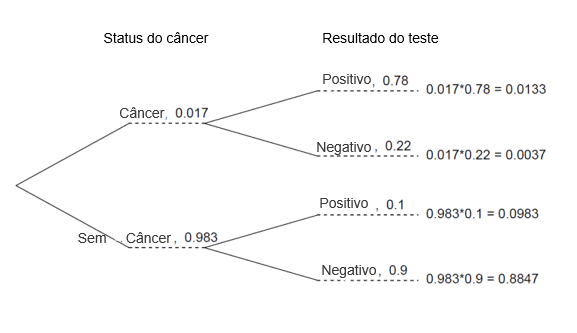
\includegraphics[width=0.9\textwidth]{2-2_conditional_probability/cancer_tree_first.png} 
}
{
\pause
{\footnotesize
\begin{eqnarray*}
&&P(C | +) \\
\pause
&&= \frac{P(C~e~+)}{P(+)} \\
\pause
&&= \frac{0.0133}{0.0133 + 0.0983} \\
\pause
&&= 0.12
\end{eqnarray*}
}
}

\pause
\justifying
\Note{Diagramas de árvores são úteis para inverter probabilidades: nos são dados $P(+|C)$ e pediu por $P(C|+)$.}

\end{frame}

%%%%%%%%%%%%%%%%%%%%%%%%%%%%%%%%%%%

\begin{frame}
\frametitle{Prática}
\justifying
\pq{Suponha que uma mulher que faça o teste uma vez obtenha um resultado positivo, se ela fizer o teste novamente, qual é a probabilidade de que essa mulher tenha câncer se essa segunda mamografia também produzir um resultado positivo?}

\twocol{0.2}{0.7}
{
\begin{enumerate}[(a)]
\item 0.0936
\item 0.088
\item 0.48
\solnMult{0.52}
\end{enumerate}
}
{
\solnGr{\only<2->{
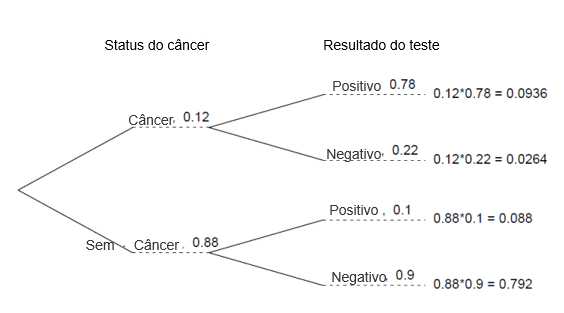
\includegraphics[width=\textwidth]{2-2_conditional_probability/cancer_tree_second.png} 
}}
}

\soln{\only<3->{
{\small \[P(C | +) = \frac{P(C~e~+)}{P(+)} = \frac{0.0936}{0.0936+0.088} = 0.52\]}
}}

\end{frame}

%%%%%%%%%%%%%%%%%%%%%%%%%%%%%%%%%%%

\subsection{Teorema de Bayes}

%%%%%%%%%%%%%%%%%%%%%%%%%%%%%%%%%%%%

\begin{frame}
\frametitle{Teorema de Bayes}

\begin{itemize}
\justifying
\item A fórmula de probabilidade condicional que vimos até agora é um caso especial do Teorema de Bayes, que também é aplicável mesmo quando os eventos têm mais de dois resultados.

\pause 
\begin{center}
    

\item \hl{Teorema de Bayes:}
\formula{
\[ P(resultado~A_1~da~variável~1~|~resultado~B~da~variável~2) \]
\[ = \frac{P(B|A_1)P(A_1)}{P(B|A_1)P(A_1) + P(B|A_2)P(A_2) + \cdots + P(B|A_k)P(A_k)} \]
}
em que $A_2$, $\cdots$, $A_k$ representam todos os outros resultados possíveis da variável 1.
\end{center}
\end{itemize}

\end{frame}

%%%%%%%%%%%%%%%%%%%%%%%%%%%%%%%%%%%

\begin{frame}
\frametitle{Atividade: invertendo probabilidades}
\justifying
\app{{\footnotesize Um modelo epidemiológico comum para a disseminação de doenças é o modelo SIR, onde a população é dividida em três grupos: Suscetível, Infectado e Recuperado. Este é um modelo razoável para doenças como catapora, onde uma única infecção geralmente fornece imunidade a infecções subsequentes. Às vezes, essas doenças também podem ser difíceis de detectar.
\vspace{2mm} \\
\justifying
Imagine uma população no meio de uma epidemia onde 60\% da população é considerada suscetível, 10\% está infectada e 30\% é recuperada. O único teste para a doença tem precisão de 95\% para indivíduos suscetíveis, 99\% para indivíduos infectados, mas 65\% para indivíduos recuperados. (Nota: Neste caso, precisão significa retornar um resultado negativo para indivíduos suscetíveis e recuperados e um resultado positivo para indivíduos infectados). \vspace{2mm} \\
Desenhe uma árvore de probabilidade para refletir as informações fornecidas acima. Se o indivíduo testou positivo, qual é a probabilidade de ele realmente estar infectado?
}}

\end{frame}

%%%%%%%%%%%%%%%%%%%%%%%%%%%%%%%%%%%

\begin{frame}
\frametitle{Atividade: invertendo probabilidades(cont.)}

\vspace{-0.5cm}

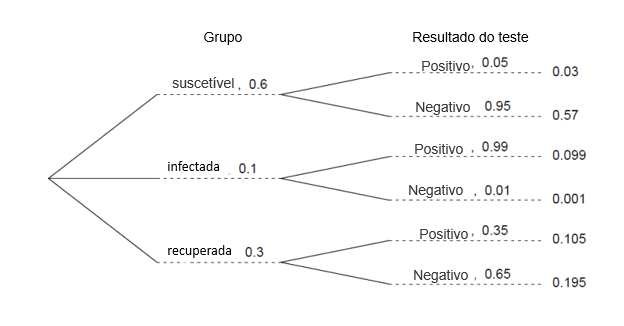
\includegraphics[width=\textwidth]{2-2_conditional_probability/sir_tree.png} 

\pause

\[ P(inf | +) = \frac{P(inf~e~+)}{P(+)} = \frac{0.099}{0.03 + 0.099 + 0.105} \approx 0.423 \]


\end{frame}

%%%%%%%%%%%%%%%%%%%%%%%%%%%%%%%%%%%%

 
%%%%%%%%%%%%%%%%%%%%%%%%%%%%%%%%%%%%

\section{2.3. Amostragem de uma população pequena}

%%%%%%%%%%%%%%%%%%%%%%%%%%%%%%%%%%%%

\begin{frame}
\frametitle{Amostragem com reposição}
\justifying
Na amostragem \hl{com reposição}, o elemento selecionado pode ser observado mais de uma vez. O elemento selecionado é devolvido à população. 

\pause

\begin{itemize}
\justifying
\item Imagine que você tenha uma caixa com 5 fichas vermelhas, 3 azuis e 2 laranjas. Qual é a probabilidade de que a primeira ficha que você tirar seja azul?

\begin{center}
5 \textcolor{red}{$\CIRCLE$}~, 3 \textcolor{blue}{$\CIRCLE$}~, 2 \textcolor{orange}{$\CIRCLE$}
\end{center}

\pause

\[ Prob(1^{0} \text{ ficha } B) = \frac{3}{5 + 3 + 2} = \frac{3}{10} = 0.3 \]

\pause
\end{itemize}

\end{frame}

%%%%%%%%%%%%%%%%%%%%%%%%%%%%%%%%%%%%

\begin{frame}
\frametitle{Amostragem com reposição}

\begin{itemize}
\justifying
\item Suponha que você realmente tenha puxado uma ficha azul da primeira vez. Usando amostragem com reposição, qual é a probabilidade de tirar uma ficha azul na segunda vez?

\pause

\begin{center}
$1^{0}$ caixa: 5 \textcolor{red}{$\CIRCLE$}~, 3 \textcolor{blue}{$\CIRCLE$}~, 2 \textcolor{orange}{$\CIRCLE$} \\

\pause

$2^{0}$ caixa: 5 \textcolor{red}{$\CIRCLE$}~, 3 \textcolor{blue}{$\CIRCLE$}~, 2 \textcolor{orange}{$\CIRCLE$}
\end{center}

\pause

\[ Prob(2^{0} \text{ ficha } B | 1^{0} \text{ ficha } B) = \frac{3}{10} = 0.3 \]

\end{itemize}

\end{frame}

%%%%%%%%%%%%%%%%%%%%%%%%%%%%%%%%%%%%%

\begin{frame}
\frametitle{Amostragem com reposição (cont.)}

\begin{itemize}
\justifying
\item Suponha que você realmente tenha puxado uma ficha laranja na primeira seleção. Usando amostragem  com reposição, qual é a probabilidade da segunda ficha ser azul?

\pause

\begin{center}
$1^{0}$ caixa: 5 \textcolor{red}{$\CIRCLE$}~, 3 \textcolor{blue}{$\CIRCLE$}~, 2 \textcolor{orange}{$\CIRCLE$} \\
\pause
$2^{0}$ caixa: 5 \textcolor{red}{$\CIRCLE$}~, 3 \textcolor{blue}{$\CIRCLE$}~, 2 \textcolor{orange}{$\CIRCLE$}
\end{center}
\pause
\[ Prob(2^{0} \text{ ficha } B | 1^{0} \text{ ficha } O) = \frac{3}{10} = 0.3 \]

\pause
\justifying
\item Se amostrar com reposição, qual é a probabilidade de selecionar duas fichas azuis?
\begin{center}

\pause
$1^{0}$ caixa: 5 \textcolor{red}{$\CIRCLE$}~, 3 \textcolor{blue}{$\CIRCLE$}~, 2 \textcolor{orange}{$\CIRCLE$} \\
$2^{0}$ caixa: 5 \textcolor{red}{$\CIRCLE$}~, 3 \textcolor{blue}{$\CIRCLE$}~, 2 \textcolor{orange}{$\CIRCLE$}
\end{center}
\pause
\vspace{0.5cm}
\[ Prob(1^{0} \text{ ficha } B) \cdot Prob(2^{0} \text{ ficha } B | 1^{0} \text{ ficha } B) = 0.3 \times 0.3 \]
\[ = 0.3^2 = 0.09 \]

\end{itemize}

\end{frame}

%%%%%%%%%%%%%%%%%%%%%%%%%%%%%%%%%%%%%

\begin{frame}
\frametitle{Amostragem com reposição (cont.)}

\begin{itemize}
\justifying
\item Ao amostrar com reposição, a probabilidade da segunda ficha ser azul não depende da cor da primeira ficha, já que qualquer item selecionado no primeiro sorteio é colocado de volta na caixa.
\[ Prob(B | B) = Prob(B | O) \]
\justifying
\item Além disso, essa probabilidade é igual à probabilidade de tirar uma ficha azul no primeiro sorteio, uma vez que a composição da caixa nunca muda quando a amostragem é feita com reposição.
\[ Prob(B | B) = Prob(B) \]
\justifying
\item \hl{Ao amostrar com reposição, os sorteios são independentes.}

\end{itemize}

\end{frame}


%%%%%%%%%%%%%%%%%%%%%%%%%%%%%%%%%%%%%

\begin{frame}
\frametitle{Amostragem sem reposição}
\justifying
Ao amostrar \hl{sem reposição}, você não coloca de volta o que acabou de selecionar.

\begin{itemize}

\pause
\justifying
\item Suponha que aprimeira fixa selecionada seja da cor azul. Se a amostra for sem reposição, qual é a probabilidade de tirar uma ficha azul na segunda vez?
\pause
\begin{center}
$1^{0}$ caixa: 5 \textcolor{red}{$\CIRCLE$}~, 3 \textcolor{blue}{$\CIRCLE$}~, 2 \textcolor{orange}{$\CIRCLE$} \\
\pause
$2^{0}$ caixa: 5 \textcolor{red}{$\CIRCLE$}~, 2 \textcolor{blue}{$\CIRCLE$}~, 2 \textcolor{orange}{$\CIRCLE$}
\end{center}
\pause
\[ Prob(2^{0} \text{ ficha } B | 1^{0} \text{ ficha } B) = \frac{2}{9} = 0.22 \]

\pause

\end{itemize}
\end{frame}

%%%%%%%%%%%%%%%%%%%%%%%%%%%%%%%%%%%%%

\begin{frame}
\frametitle{Amostragem sem reposição (cont.)}

\begin{itemize}
\justifying
\item Se a amostragem for sem reposição, qual é a probabilidade de selecionar duas fichas azuis?
\begin{center}

\pause
$1^{0}$ caixa: 5 \textcolor{red}{$\CIRCLE$}~, 3 \textcolor{blue}{$\CIRCLE$}~, 2 \textcolor{orange}{$\CIRCLE$} \\
$2^{0}$ caixa: 5 \textcolor{red}{$\CIRCLE$}~, 2 \textcolor{blue}{$\CIRCLE$}~, 2 \textcolor{orange}{$\CIRCLE$}
\end{center}
\pause
\[ Prob(1^{0} \text{ ficha } B) \cdot Prob(2^{0} \text{ ficha } B | 1^{0} \text{ ficha } B)  = 0.3 \times 0.22 \]
\[ = 0.066 \]

\end{itemize}

\end{frame}

%%%%%%%%%%%%%%%%%%%%%%%%%%%%%%%%%%%%%

\begin{frame}
\frametitle{Amostragem sem reposição (cont.)}

\begin{itemize}
\justifying
\item Ao amostrar sem reposição, a probabilidade da segunda ficha ser azul dado que a primeira foi azul não é igual à probabilidade de amostrar uma ficha azul no primeiro sorteio, já que a composição da caixa muda com o resultado do primeiro sorteio.
\[ Prob(B | B) \ne Prob(B) \]

\pause
\justifying
\item \hl{Ao amostrar sem reposição, os sorteios não são independentes.}

\pause
\justifying
\item Isso é especialmente importante quando os tamanhos das populações que são amostradas são pequenas. Se estivéssemos lidando com, digamos, 10.000 fichas em uma caixa (gigante), tirar uma ficha de qualquer cor não teria um impacto tão grande nas probabilidades no segundo sorteio.

\end{itemize}

\end{frame}

%%%%%%%%%%%%%%%%%%%%%%%%%%%%%%%%%%%%%

\begin{frame}
\frametitle{Prática}
\justifying
\pq{Na maioria dos jogos de cartas, as cartas são distribuídas sem reposição. Qual é a probabilidade de receber um ás e depois um 3? Escolha a resposta mais próxima.}

\twocol{0.3}{0.6}{
\begin{enumerate}[(a)]
\item 0.0045
\item 0.0059
\solnMult{0.0060}
\item 0.1553
\end{enumerate}
}
{
\soln{
\pause
\[ P(ás~então~3) = \frac{4}{52} \times \frac{4}{51} \approx 0.0060 \]
}}

\end{frame}

%%%%%%%%%%%%%%%%%%%%%%%%%%%%%%%%%%%%%

 
%%%%%%%%%%%%%%%%%%%%%%%%%%%%%%%%%%%%

\section{2.4. Variáveis aleatórias}

%%%%%%%%%%%%%%%%%%%%%%%%%%%%%%%%%%%%

\begin{frame}
\frametitle{Variáveis aleatórias}

\begin{itemize}
\justifying
\item Uma \hl{variável aleatória} é uma quantidade numérica cujo valor depende do resultado de um evento aleatório.
\begin{itemize}
\justifying
\item Usamos uma letra maiúscula, como $ X $, para denotar uma variável aleatória.
\justifying
\item Os valores de uma variável aleatória são denotados com uma letra minúscula, neste caso $ x $.
\justifying
\item Por exemplo, $P(X = x)$.
\end{itemize}
\justifying
\item Existem dois tipos de variáveis aleatórias:
\begin{itemize}
\justifying
\item \hl{Variáveis aleatórias discretas} representam valores inteiros.
\begin{itemize}
\justifying
\item Exemplo: Número de filhos, número de carros, número de clientes de uma loja,...
\end{itemize}
\justifying
\item \hl{Variáveis aleatórias contínuas} valores reais
\begin{itemize}
\justifying
\item Exemplo: Preço de um livro, peso, altura, tempo...
\end{itemize}
\end{itemize}

\end{itemize}

\end{frame}

%%%%%%%%%%%%%%%%%%%%%%%%%%%%%%%%%%%%

\subsection{Esperança}

%%%%%%%%%%%%%%%%%%%%%%%%%%%%%%%%%%%%

\begin{frame}
\frametitle{Esperança}

\begin{itemize}
\justifying
\item Estamos frequentemente interessados no resultado médio de uma variável aleatória.
\justifying
\item Chamamos isso de \hl{valor esperado} (média). A média é uma soma ponderada dos possíveis resultados.\\
\formula{\[\mu = E(X) = \sum_{i = 1}^k x_i ~ P(X = x_i)\]}

\end{itemize}

\end{frame}

%%%%%%%%%%%%%%%%%%%%%%%%%%%%%%%%%%%%

\begin{frame}
\frametitle{Valor esperado de uma variável aleatória discreta}
\justifying
\dq{Em um jogo de cartas, você ganha \$ 1 se tirar um coração, \$ 5 se você comprar um ás (incluindo o ás de copas), \$ 10 se você tirar o rei de espadas e nada para qualquer outra carta que você selecionar. Escreva o modelo de probabilidade para seus ganhos e calcule seu ganho esperado.}

\pause

\begin{center}
\scalebox{0.85}{
\renewcommand{\arraystretch}{1.5}
\begin{tabular}{l | c | c | c }
Evento		& $X$ 		& $P(X)$        		& $X ~ P(X)$ \\
\hline
Coração (não de ás)	& $1$		& $\frac{12}{52}$	& $\frac{12}{52}$ \\
Ás			& $5$		& $\frac{4}{52}$	& $\frac{20}{52}$ \\	
Rei de espadas	& $10$		& $\frac{1}{52}$	& $\frac{10}{52}$ \\	
Todos os outros		& $0$		& $\frac{35}{52}$	& $0$ \\
\hline
Total			&			&				& $E(X) = \frac{42}{52} \approx 0.81$
\end{tabular}
}
\end{center}

\end{frame}

%%%%%%%%%%%%%%%%%%%%%%%%%%%%%%%%%%%%

\begin{frame}
\frametitle{Valor esperado de uma variável aleatória discreta (cont.)}
\justifying
Abaixo está uma representação visual da distribuição de probabilidade dos ganhos deste jogo:

\begin{center}
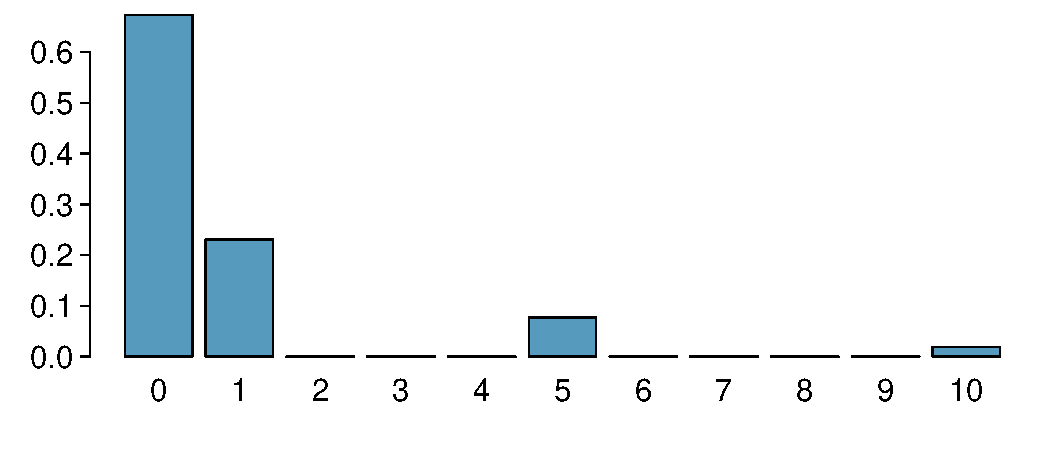
\includegraphics[width=0.8\textwidth]{2-4_random_variables/card_game.pdf}
\end{center}

\end{frame}

%%%%%%%%%%%%%%%%%%%%%%%%%%%%%%%%%%%%

\subsection{Variância de variáveis aleatórias}

%%%%%%%%%%%%%%%%%%%%%%%%%%%%%%%%%%%%

\begin{frame}
\frametitle{Variância}
\justifying
Também estamos frequentemente interessados na variabilidade dos valores de uma variável aleatória.

\formula{
\[ \sigma^2 = Var(X) = \sum_{i = 1}^k (x_i - E(X))^2 P(X = x_i) \]
\[ \sigma = SD(X) = \sqrt{Var(X)} \]
}

\end{frame}

%%%%%%%%%%%%%%%%%%%%%%%%%%%%%%%%%%%%

\begin{frame}
\frametitle{Variância de uma variável aleatória discreta}
\justifying
\dq{Para o exemplo anterior do jogo de cartas, quanto você esperaria que os ganhos variassem de jogo para jogo?}

\vspace{2mm}
\only<2->{

\scalebox{0.75}{
\begin{center}
\renewcommand{\arraystretch}{2}
\begin{tabular}{c | c | c | l | p{4cm}}
$X$ & $P(X)$         & $X ~ P(X)$      & \multicolumn{1}{c|}{$(X - E(X))^2$}  & \multicolumn{1}{c}{$P(X) ~ (X - E(X))^2$}  \\
\hline
1 & $\frac{12}{52}$  & $1 \times \frac{12}{52} = \frac{12}{52}$ & $(1 - 0.81)^2 = 0.0361$ &  $\frac{12}{52} \times 0.0361 = 0.0083$ \\
\hline
5 & $\frac{4}{52}$   & $5 \times \frac{4}{52} = \frac{20}{52}$ & $(5 - 0.81)^2 = 17.5561$  & $\frac{4}{52} \times 17.5561 = 1.3505$ \\
\hline
10  & $\frac{1}{52}$ & $10 \times \frac{1}{52} = \frac{10}{52}$  & $(10 - 0.81)^2 = 84.4561$   & $\frac{1}{52} \times 84.0889 = 1.6242$ \\
\hline
0 & $\frac{35}{52}$  & $0 \times \frac{35}{52} = 0$  & $(0 - 0.81)^2 = 0.6561$ & $\frac{35}{52} \times 0.6561 = 0.4416$ \\
\hline
  &       & $E(X) = 0.81$ & & \soln{\only<3->{$V(X) = 3.4246$}} \\
 &       &                                                         & & \soln{\only<4>{$SD(X) = \sqrt{3.4246} = 1.85$}} \\
\end{tabular}
\end{center}
}
}
\end{frame}

%%%%%%%%%%%%%%%%%%%%%%%%%%%%%%%%%%%%

\subsection{Combinações lineares de variáveis aleatórias}

%%%%%%%%%%%%%%%%%%%%%%%%%%%%%%%%%%%%

\begin{frame}
\frametitle{Combinações lineares}

\begin{itemize}
\justifying
\item Uma \hl {combinação linear} de variáveis aleatórias $ X $ e $ Y $ é dada por\\

\[ aX + bY \]

onde $a$ e $b$ são alguns números fixos.

\pause
\justifying
\item O valor médio de uma combinação linear de variáveis aleatórias é dado por\\
\formula{\[ E(aX + bY) = a \times E(X) + b \times E(Y) \]}

\end{itemize}

\end{frame}

%%%%%%%%%%%%%%%%%%%%%%%%%%%%%%%%%%%%

\begin{frame}
\frametitle{Calculando a esperança de uma combinação linear}
\justifying
\dq{Imagine que em média, você leva 10 minutos para fazer um exercício de estatística e 15 minutos para terminar um exercício de física. Esta semana você deve fazer uma lista com 5 exercícios de estatística e um trabalho com 4 exercícios de física. Qual o tempo total que você espera gastar para fazer as duas tarefas?}\\

\soln{
\pause
\begin{align*} 
E(Est + Est + Est + Est + Est + Fis + Fis + Fis + Fis) &= 5 \times E(Est) + 4 \times E(Fis) \\
&= 5 \times 10 + 4 \times 15 \\
&= 50 + 60 \\
&= 110~min 
\end{align*}
}

\end{frame}

%%%%%%%%%%%%%%%%%%%%%%%%%%%%%%%%%%%%

\subsection{Variância de combinações lineares de variáveis aleatórias}

%%%%%%%%%%%%%%%%%%%%%%%%%%%%%%%%%%%%

\begin{frame}
\frametitle{Combinações lineares}

\begin{itemize}
\justifying
\item A variância de uma combinação linear de duas variáveis aleatórias independentes é\\
\formula{\[ V(aX + bY) = a^2 \times V(X) + b^2 \times V(Y) \]}

\pause 
\justifying
\item O desvio padrão da combinação linear é a raiz quadrada da variância.

\pause 

\justifying
\item Se as variáveis aleatórias não forem independentes, o cálculo da variância fica um pouco mais complicado\\
\formula{\[ V(aX + bY) = a^2 \times V(X) + b^2 \times V(Y) + 2abCov(X, Y) \]}


\end{itemize}

\end{frame}

%%%%%%%%%%%%%%%%%%%%%%%%%%%%%%%%%%%%

\begin{frame}
\frametitle{Calculando a variância de uma combinação linear}
\justifying
\dq{O desvio padrão do tempo que você leva para cada problema de estatística é 1,5 minutos, e é de 2 minutos para cada problema de física. Qual é o desvio padrão do tempo que você espera gastar? Suponha que o tempo para resolver cada exercício seja independente do outro.}\\

\soln{
\pause
\small{
\begin{align*} 
V(Est + Est + Est + Est + Est + Fis + Fis + Fis + Fis) &= V(Est) + V(Est) + V(Est) + V(Est) + V(Est)  \\
& + V(Fis) + V(Fis) + V(Fis) + V(Fis) \\
&= 5 \times V(Est) + 4 \times V(Fis) \\
&= 5 \times 1.5^2 + 4 \times 2^2 \\
&= 27.25
\end{align*}
}}

\end{frame}

%%%%%%%%%%%%%%%%%%%%%%%%%%%%%%%%%%%%

\subsection{Relembrando}

%%%%%%%%%%%%%%%%%%%%%%%%%%%%%%%%%%%%

\begin{frame}
\frametitle{Prática}
\justifying
\pq{Um jogo de cartas em um cassino custa \$5 por partida. Se a primeira carta que você tirar for vermelha, você poderá comprar uma segunda carta (sem substituição). Se a segunda carta é o ás de paus, você ganha \$500. Se não, você não ganha nada, ou seja, perde os \$5. Qual é o lucro/prejuízo esperado ao jogar este jogo? {\small Lembre-se: lucro/perda = ganhos - custo.}}


\begin{multicols}{2}
\begin{enumerate}[(a)]
\item Um lucro de 5\$
\solnMult{Uma perda de 10\$}
\item Uma perda de 25\$
\item Uma perda de 30\$
\end{enumerate}
\end{multicols}

\vspace{-1cm}



\begin{table}[!h]\footnotesize
\scriptsize
\centering
\begin{tabular}{l c c c r}
Evento				& Ganho	& Lucro: $X$	& $P(X)$	& $ X \times P(X)$	\\
\hline
\orange{Vermelho}, {A}{$\clubsuit$}		& 500		& 500 - 5 = 495	& $\frac{26}{52} \times \frac{1}{51} = 	0.0098$ & 	 $495 \times 0.0098 = 4.851$ \\
Outros	& 0 			& 0 - 5 = -5	& $1 - 0.0098 = 0.9902$ & $-5 \times 0.9902 = -4.951$ \\  
\hline
					&			&			& 			& $E(X) = -0.1$
\end{tabular}
\end{table}


\end{frame}

%%%%%%%%%%%%%%%%%%%%%%%%%%%%%%%%%%%%

\begin{frame}
\frametitle{Jogo Justo}
\justifying
Um jogo \hl{justo} é definido como um jogo em que o custo e o prêmio esperado são iguais, ou seja, o lucro esperado é 0.

\pause

$\:$
\justifying
\dq{Você acha que os jogos nos cassinos em Vegas custam mais ou menos do que os ganhos esperados?}

\soln{
\pause
\begin{columns}[c]
\column{0.6\textwidth}
\justifying
Se esses jogos custassem menos do que o esperado, isso significaria que em médias os cassinos perderiam dinheiro:
\column{0.4\textwidth}
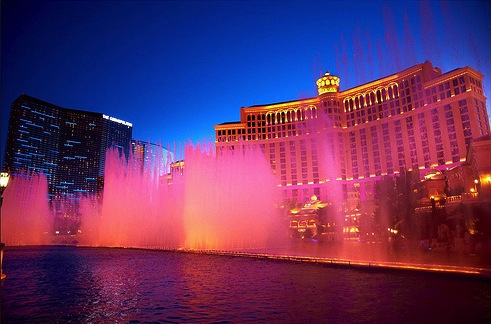
\includegraphics[width=\textwidth]{2-4_random_variables/bellagio.jpg}
\end{columns}
\ct{Image by Moyan\_Brenn on Flickr \webURL{http://www.flickr.com/photos/aigle\_dore/5951714693}.}
}


\end{frame}

%%%%%%%%%%%%%%%%%%%%%%%%%%%%%%%%%%%%%

\begin{frame}
\frametitle{Propriedades de Variáveis Aleatórias}
\justifying
Variáveis aleatórias não funcionam como variáveis algébricas:\\
\[ X + X \ne 2X \]

\pause

{\small
\twocol{0.45}{0.45}
{
\begin{align*}
E(X + X) &= E(X) + E(X) \\
&= 2 E(X) \\
&~  \\
E(2X) &= 2 E(X) \\
&~ 
\end{align*}
}
{
\begin{align*}
Var(X + X) &= Var(X) + Var(X)~{\scriptsize \text{(assumindo independência)}} \\
&= 2~Var(X) \\
&~  \\
Var(2X) &= 2^2~Var(X) \\
&= 4~Var(X)
\end{align*}
}
}


\pause

\vspace{3mm}

\mathhl{E(X + X)  = E(2X)}, mas \mathhl{Var(X + X) \ne Var(2X)}.

\end{frame}

%%%%%%%%%%%%%%%%%%%%%%%%%%%%%%%%%%%%%

\begin{frame}
\frametitle{Adicionando ou multiplicando?}
\justifying
\dq{Uma empresa tem 5 carros em sua frota, aados históricos mostram que o custo anual de manutenção para cada carro é, em média, de \$ 2.154 com um desvio padrão de \$ 132. Qual é a média e o desvio padrão do custo total anual de manutenção para esta frota ?}

\pause
\justifying
Note que temos 5 carros, cada um com custo anual de manutenção $(X_1 + X_2 + X_3 + X_4 + X_5)$.

\pause
\end{frame}
%%%%%%%%%%%%%%%%%%%%%%%%%%%%%%%%%%%%%

\begin{frame}
\frametitle{Adicionando ou multiplicando?}

\scalefont{0.8}
\begin{eqnarray*} 

E(X_1 + X_2 + X_3 + X_4 + X_5) &=& E(X_1) + E(X_2) + E(X_3) + E(X_4) + E(X_5) \\
\pause

&=& 5 \times E(X) = 5 \times 2,154 = \$ 10,770 \\
\pause

Var(X_1 + X_2 + X_3 + X_4 + X_5) &=& Var(X_1) + Var(X_2) + Var(X_3) + Var(X_4) + Var(X_5) \\
\pause

&=& 5 \times V(X) = 5 \times 132^2 = \$ 87,120 \\
\pause

SD(X_1 + X_2 + X_3 + X_4 + X_5) &=& \sqrt{87,120} =  295.16

\end{eqnarray*}


\end{frame}
%%%%%%%%%%%%%%%%%%%%%%%%
 
%%%%%%%%%%%%%%%%%%%%%%%%%%%%%%%%%%%%

\section{2.5. Distribuições contínuas}

%%%%%%%%%%%%%%%%%%%%%%%%%%%%%%%%%%%%

\begin{frame}
\frametitle{Distribuições contínuas}

\begin{itemize}
\justifying
\item Abaixo um histograma da distribuição da altura de adultos. 
\justifying
\item A proporção de dados que cai nas caixas sombreadas dá a probabilidade de um adulto amostrado aleatoriamente ter entre 180cm e 185cm.

\end{itemize}

\begin{center}
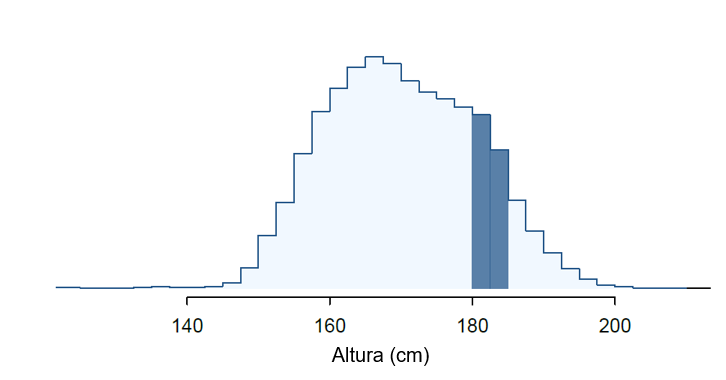
\includegraphics[width=0.75\textwidth]{2-5_continuous_distributions/usHeightsHist180185.png}
\end{center}


\end{frame}

%%%%%%%%%%%%%%%%%%%%%%%%%%%%%%%%%%%%

\subsection{Histogramas de distribuições contínuas}

\begin{frame}
\frametitle{Histogramas de distribuições contínuas}
\justifying
Como a altura é uma variável numérica contínua, sua \hl{função densidade de probabilidade} é uma curva suave.

\begin{center}
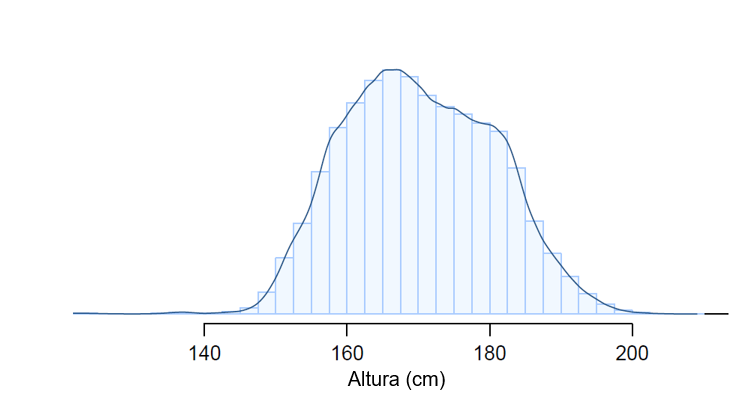
\includegraphics[width=\textwidth]{2-5_continuous_distributions/fdicHeightContDist.png}
\end{center}

\end{frame}

%%%%%%%%%%%%%%%%%%%%%%%%%%%%%%%%%%%%

\subsection{Distribuições contínuas}

\begin{frame}
\frametitle{Probabilidades de distribuições contínuas}
\justifying
A probabilidade de um adulto selecionado aleatoriamente ter entre 180cm e 185cm também pode ser estimada como a área sombreada sob a curva.

\begin{center}
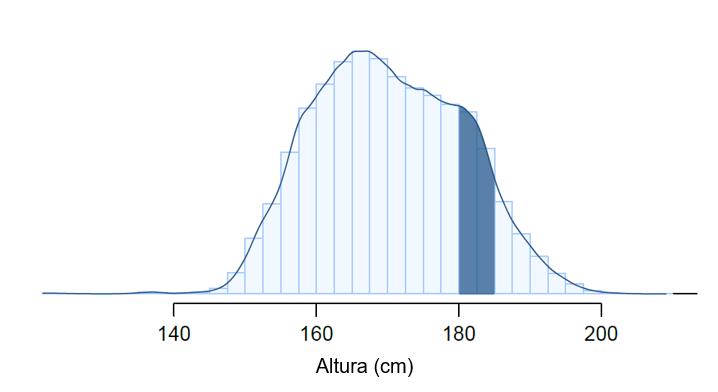
\includegraphics[width=\textwidth]{2-5_continuous_distributions/fdicHeightContDistFilled.png}
\end{center}


\end{frame}

%%%%%%%%%%%%%%%%%%%%%%%%%%%%%%%%%%%%

\begin{frame}
\frametitle{Por definição...}
\justifying
A probabilidade é estimada como "a área sob a curva", a probabilidade de uma pessoa ter exatamente 180cm (ou qualquer valor exato) é definida como 0.

\begin{center}
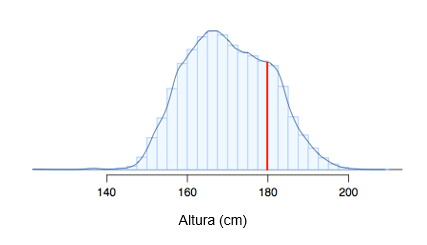
\includegraphics[width=0.8\textwidth]{2-5_continuous_distributions/fdicHeightContDist180.png}
\end{center}

\end{frame}

%%%%%%%%%%%%%%%%%%%%%%%%%%%%%%%%%%%%
 


%%%%%%%%%%%%%%%%%%%%%%%%%%%%%%%%%%%%
% End document
%%%%%%%%%%%%%%%%%%%%%%%%%%%%%%%%%%%%

\end{document}